\documentclass[tikz,border=3pt]{standalone}
\usetikzlibrary{arrows.meta,fit,backgrounds}
\definecolor{ink}{HTML}{344451}
\definecolor{blue}{HTML}{426C8B}
\definecolor{pale}{HTML}{EFF5F8}
\definecolor{accent}{HTML}{88506D}
\definecolor{orange}{HTML}{BA8243}
\newcommand{\sub}{\fontsize{9}{10}\selectfont}
\begin{document}
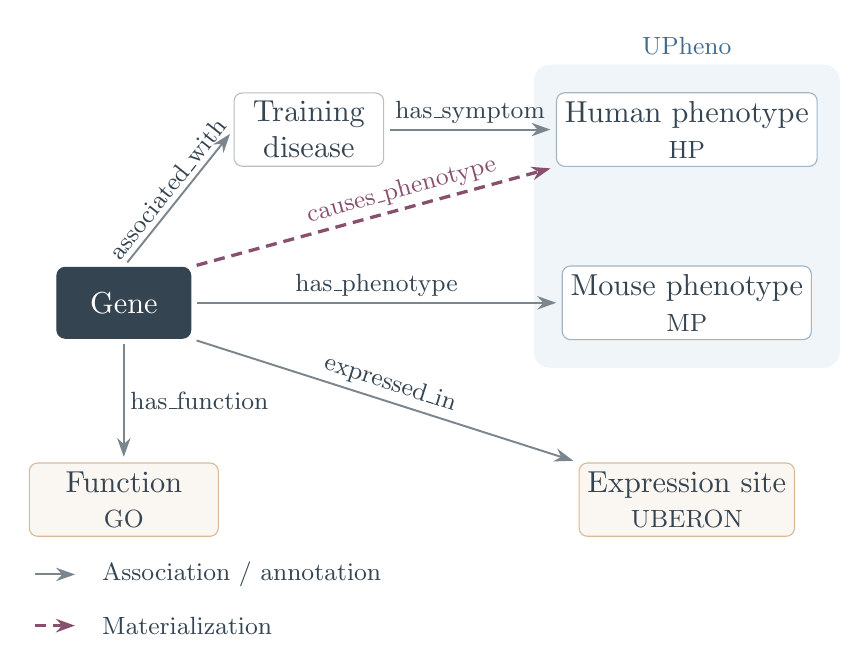
\begin{tikzpicture}[
 font=\fontsize{11}{13}\selectfont,text=ink,
 >={Stealth[length=2.4mm,width=1.7mm]},
 entity/.style={rounded corners=3pt,draw=ink!35,fill=white,minimum height=9mm,minimum width=19mm,align=center,inner sep=3pt},
 pheno/.style={entity,draw=blue!50,fill=white,minimum width=23mm},
 label/.style={font=\fontsize{9.5}{11}\selectfont,inner sep=2pt},
 legend/.style={font=\fontsize{9.5}{11}\selectfont},
 edge/.style={->,draw=ink!65,line width=.7pt,shorten >=2pt,shorten <=2pt},
 material/.style={->,draw=accent,line width=1.2pt,dash pattern=on 4pt off 2.5pt,shorten >=2pt,shorten <=2pt}
]
\node[entity,fill=ink,text=white,draw=ink,minimum width=17mm] (gene) at (0,0) {Gene};
\node[entity] (disease) at (2.35,2.2) {Training\\disease};
\node[pheno] (hp) at (7.15,2.2) {Human phenotype\\{\sub HP}};
\node[pheno] (mp) at (7.15,0) {Mouse phenotype\\{\sub MP}};
\node[entity,fill=orange!7,draw=orange!55,minimum width=24mm] (go) at (0,-2.5) {Function\\{\sub GO}};
\node[entity,fill=orange!7,draw=orange!55,minimum width=24mm] (anatomy) at (7.15,-2.5) {Expression site\\{\sub UBERON}};
\begin{scope}[on background layer]
\node[fill=pale,rounded corners=6pt,inner xsep=8pt,inner ysep=10pt,fit=(hp)(mp)] (upheno) {};
\end{scope}
\node[anchor=south,legend,text=blue] at (upheno.north) {UPheno};
\draw[edge] (gene.north) -- node[label,above,sloped] {associated\_with} (disease.west);
\draw[edge] (disease.east) -- node[label,above] {has\_symptom} (hp.west);
\draw[edge] (gene.east) -- node[label,above] {has\_phenotype} (mp.west);
\draw[edge] (gene.south) -- node[label,right] {has\_function} (go.north);
\draw[edge] (gene.south east) -- node[label,above,sloped] {expressed\_in} (anatomy.north west);
\draw[material] (gene.north east) -- node[label,above,sloped,pos=.59,text=accent] {causes\_phenotype} (hp.south west);
\draw[edge] (-1.2,-3.45) -- (-.55,-3.45);
\node[anchor=west,legend] at (-.4,-3.45) {Association / annotation};
\draw[material] (-1.2,-4.1) -- (-.55,-4.1);
\node[anchor=west,legend] at (-.4,-4.1) {Materialization};
\end{tikzpicture}
\end{document}
